\begin{blocksection}
\question Fill in each blank in the code example below so that its environment diagram is the following. You do not need to use all the blanks.

\begin{multicols}{2}
\begin{lstlisting}
fruit = [1, 2, [3, 4]]
fruit._______________________
fruit[3][2]._________________
fruit[2][2]._________________
fruit[3][3][2][2][2][1] = ___
\end{lstlisting}

\columnbreak
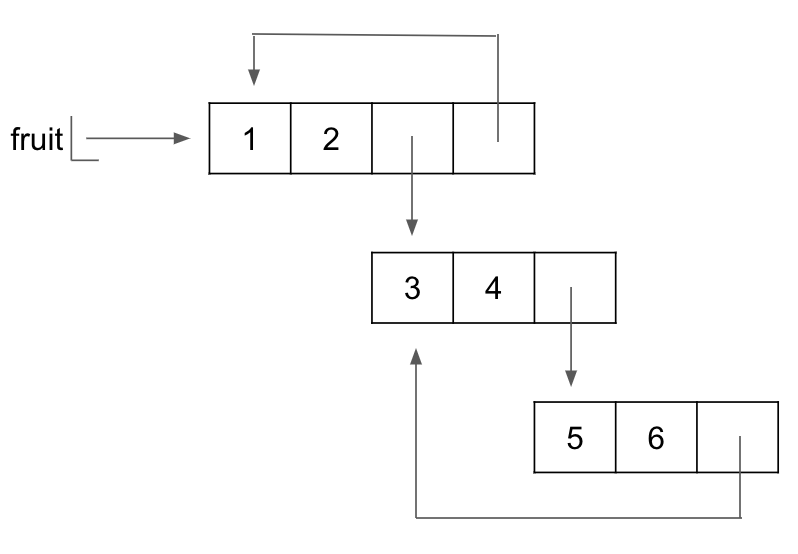
\includegraphics[width=.45\textwidth]{fruit_loops.png}
\end{multicols}

\begin{solution}[2in]
\begin{lstlisting}
fruit = [1, 2, [3, 4]]
fruit.append(fruit)
fruit[3][2].append([5, 6])
fruit[2][2].append(fruit[2])
fruit[3][3][2][2][2][1] = 4
\end{lstlisting}
\end{solution}
\end{blocksection}

\begin{blocksection}
\begin{guide}
\textbf{Teaching Tips}
\begin{itemize}
	\item So many nested lists!! Be very clear when you are explaining these concepts to your students and when you are drawing as it's very easy to get confused.
	\item Review with students how to use arrows in list diagrams, such as shallow and deep copies, values vs. references.
	\item The best way to approach this problem is to just go line by line, counting the indices as you go. Remember to make the distinction between reassigning what an arrow in a box points to and updating the value of the box itself (to a value or to another arrow). (This is also good practice for 61B)
	\item If your students get stuck, a good hint would be to tell them that they do indeed need all the blanks. Do not try to squeeze too many operations into one line.
\end{itemize}
\end{guide}
\end{blocksection}
